\begin{frame}
\frametitle{Analyse}
%\vspace*{-0.5cm}
\begin{columns}
\begin{column}{0.65\textwidth}
\begin{maliste}
\item Bruits de fond "physiques" : \\
\begin{small}
\textcolor{blue}{$t\bar{t}W/Z$, Dibosons, $t\bar{t}H$, $t\bar{t}WW$, $WH$, $ZH$, $WWW^*$, $ZWW^*$, $tWZ$, $tH$}
\end{small}
\vspace*{0.2cm}
\item Bruits de fond "instrumentaux" : 
\begin{small}
\begin{itemize}
\item \textcolor{blue}{\english{fakes} :} semi-leptonic $b$ decay, $\pi^0$, etc.
\item \textcolor{blue}{\english{Q Mis-id} :} mauvaise reconstruction charge
\end{itemize}
\end{small}
\vspace*{0.2cm}
\item R\'egions de signal :
\end{maliste}

\begin{table}[!htb]
        \begin{center}
\hspace*{-0.8cm}
        \scalebox{0.7} {
        \begin{tabular}{ c | c | c | c }
        \hline
        \multicolumn{3}{c|}{D\'efinition} & Nom \\
        \hline
        \multirow{2}{*}{$400~< H_T < 700~$GeV}               & \multicolumn{2}{c|}{$N_b = 2$} &  SR4t0 \\
        \cline{2-4}
                                        & \multicolumn{2}{c|}{$N_b \geq 3$} &SR4t1 \\
        \hline
        \multirow{3}{*}{$H_T \geq 700~$GeV}                    & \multirow{2}{*}{$N_b = 2$}                            & $40~< \hbox{\met} < 100~$GeV                 &  SR4t2 \\
        \cline{3-4}
                                                                                         &                                                                      & $\hbox{\met}\geq 100~$GeV                                    &  SR4t3 \\
        \cline{2-4}
                                                                                        &  \multicolumn{2}{c|}{$N_b \geq 3$} & SR4t4 \\
        \hline
\end{tabular}
%\caption{D\'efinitions des cat\'egories utilis\'ees pour d\'efinir les r\'egions de signal.\label{tab:allSR}}
}
\end{center}
\end{table} 

\end{column}
\begin{column}{0.35\textwidth}

\begin{center}
\hspace*{-0.5cm}
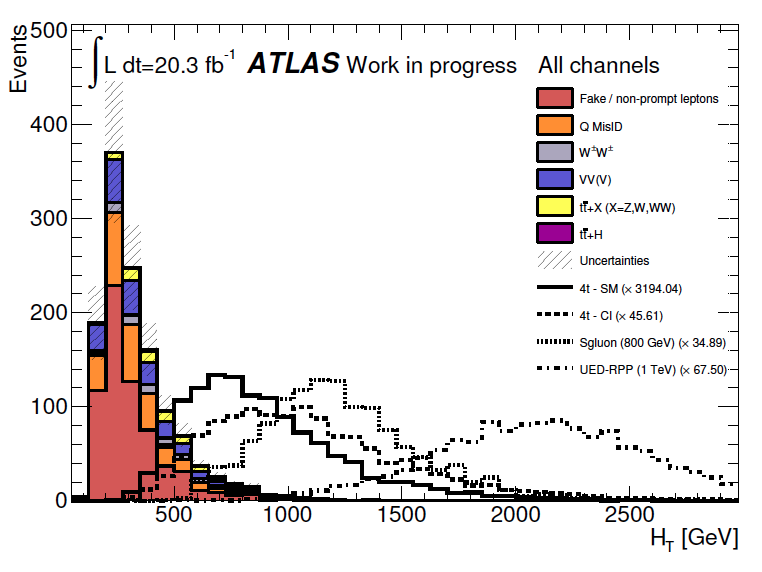
\includegraphics[width=1.2\textwidth]{Figures/FourTops/HTDistrib4topSignals.png}\\
\hspace*{-0.5cm}
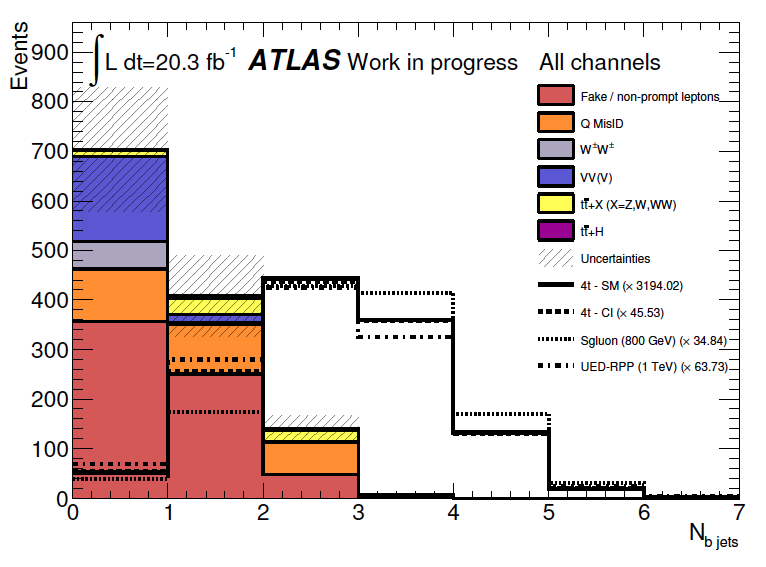
\includegraphics[width=1.2\textwidth]{Figures/FourTops/NbJetsDistrib4topSignals.png}
\end{center}

\end{column}
\end{columns}
\end{frame}

\begin{frame}
\frametitle{Résultats}

\begin{columns}
\begin{column}{0.7\textwidth}
\begin{center}
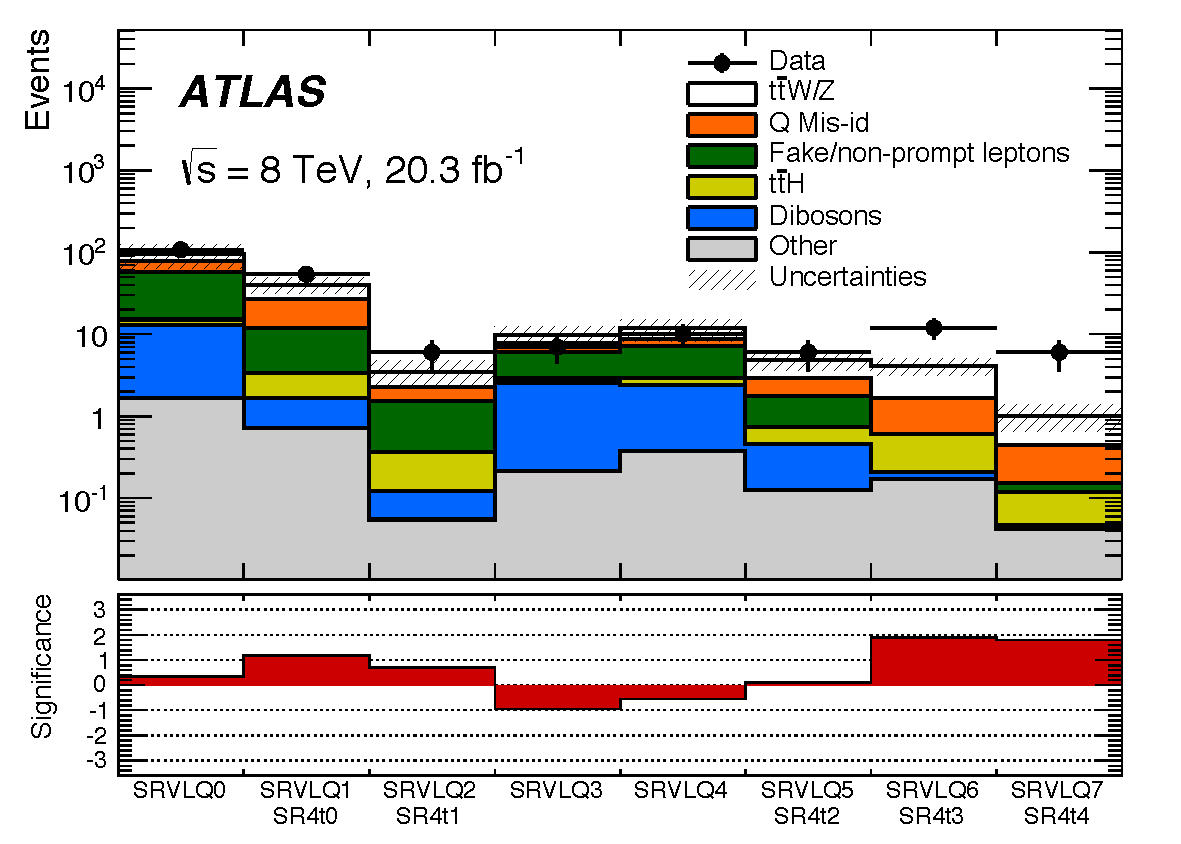
\includegraphics[width=1\textwidth]{Figures/FourTops/ExpectedBackgroundObeservedCategories.pdf}
\end{center}
\end{column}
\begin{column}{0.45\textwidth}
\begin{small}
\begin{maliste}
\item Incertitudes syst\'ematiques
\begin{itemize}
\item sections efficaces $t\bar{t}W/Z$, Dibosons, etc.
\item statistique (taille finie \'echantillons)
\item JES
\item b-tag
\item taux \english{fakes}
\item taux \english{Q Mis-id}
\item etc.
\end{itemize}
\end{maliste}
\end{small}
\end{column}
\end{columns}
\end{frame}

\begin{frame}
\frametitle{R\'esultats}

\begin{center}
\hspace*{-1cm}
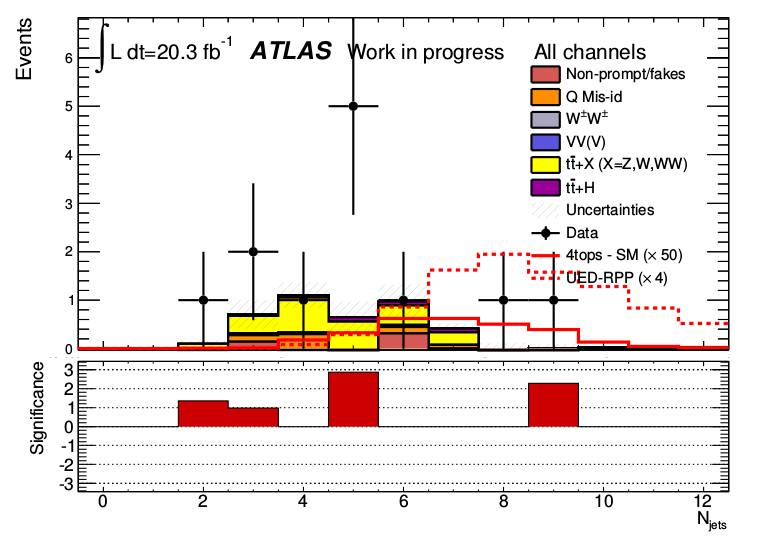
\includegraphics[width=0.58\textwidth]{Figures/FourTops/Njets_SR4t3.png}
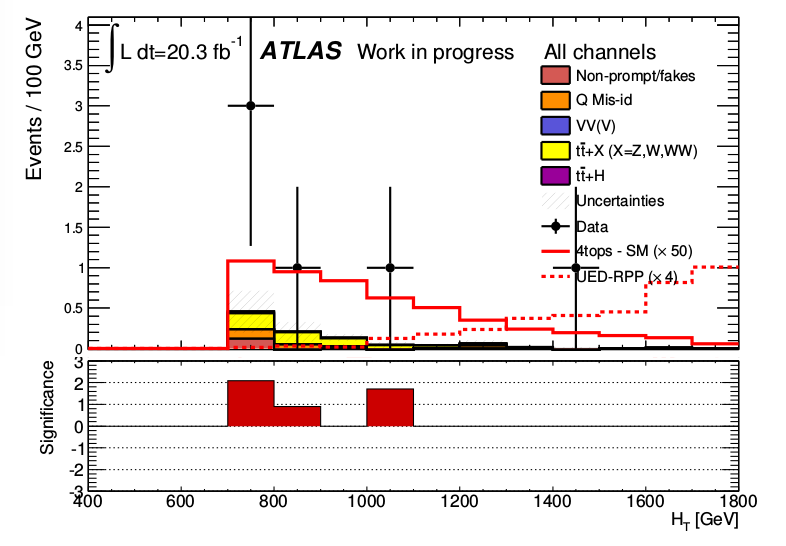
\includegraphics[width=0.595\textwidth]{Figures/FourTops/HT_SR4t4.png}
\put(-280,130){\footnotesize{SR4t3}}
\put(-100,130){\footnotesize{SR4t4}}
\end{center}

\begin{small}
\begin{maliste}
\item V\'erifications :
\begin{itemize}
\item Validation des fonds dans des r\'egions de contr\^ole 
\item Estimation des fonds par des m\'ethodes alternatives
\item Qualit\'e des objets
\item R\'epartition des \'ev\'enements observ\'es au cours du temps
\end{itemize}
%\item \textcolor{red}{commentaire sur l'exces}
%\item Plots pour dire que ca ressemble ni a l'interaction de contact ni au RPP (ni au sgluon ou au SM ?)
%\item Resumer les propriétés principales et les etudes qui ont ete faites pour ``valider'' l'exces (id des leptons, b-tagging, validation des fonds)
\end{maliste}
\end{small}
\end{frame}

